\chapter{接触网机械计算}

\section{负载计算}
由原始资料可知,站线和正线均采用JT-95型承力索。对于接触线,站线选用CT-110型接触线,正线选用CT-120型接触线。

查阅相关数据表可知JT-95承力索的单位自重为:
$$
g_c=0.849\times 9.81\times 10^{-3}=8.33\times 10^{-3}\mathrm{ }k{{N}/{m}}
$$

CT-110接触线的单位自重为:
$$
g_{j110}=0.992\times 9.81\times 10^{-3}=9.73\times 10^{-3}\mathrm{ }k{{N}/{m}}
$$

CT-120接触线的单位自重为:
$$
g_{j120}=1.082\times 9.81\times 10^{-3}=10.61\times 10^{-3}\mathrm{ }k{{N}/{m}}
$$

根据经验,吊弦及吊弦线夹的单位自重取为:
$$
g_d=0.5\times 10^{-3}k{{N}/{m}}
$$

\subsection{线索单位纯覆冰荷载}
(1)承力索单位纯覆冰荷载:

承力索的单位纯覆冰荷载计算式为:
$$
g_{cb}=\pi \gamma _bb(b+d)g_H\times 10^{-9}
$$
上式中,$g_{cb}$为承力索的单位纯冰重量,$kN/m$;$b$为承力索标准覆冰厚度,$mm$;$ $d为承力索标称直径,$mm$;$g_H$为重力加速度,取为$9.81m/s^2$;γb为覆冰密度,取为$900kg/m^3$。

由原始资料可知,气象区VIII的标准覆冰厚度为10mm,JT-95承力索的标称直径为12.5mm,计算可得JT-95承力索单位纯覆冰荷载为:
\begin{align}
	g_{cb}&=\pi \gamma _bb(b+d)g_H\times 10^{-9}\notag
	\\
	&=3.14\times 900\times 10\times \left( 10+12.5 \right) \times 9.81\times 10^{-9}\notag
	\\
	&=6.24\times 10^{-3}\notag
\end{align}
(2)接触线单位纯覆冰荷载:

接触线的单位纯覆冰荷载计算式为:
$$
g_{jb}=\pi \gamma _b\frac{b}{2}(\frac{b}{2}+\frac{A+B}{2})g_H\times 10^{-9}
$$
上式中,$g_{jb}$为接触线的单位纯冰重量,$kN/m$;A、B为接触线横断面的高度和宽度,$mm$;其余符号的物理意义与承力索单位纯覆冰荷载计算式相同。
由原始资料可知,CT-120的接触线横断面的高度和宽度分别为12.9mm和12.9mm,CT-110的接触线横断面的高度和宽度均为12.34mm。因此,对于站线,CT-110接触线单位纯覆冰荷载为:
\begin{align}
g_{jb110}&=\pi \gamma _b\frac{b}{2}\left( \frac{b}{2}+\frac{A+B}{2} \right) g_H\times 10^{-9}\notag
\\
&=3.14\times 900\times 5\times \left( 5+\frac{12.34+12.34}{2} \right) \times 9.81\times 10^{-9}\notag
\\
&=2.405\times 10^{-3}kN/m\notag
\end{align}

对于正线,CT-120接触线单位纯覆冰荷载为:
\begin{align}
g_{jb120}&=\pi \gamma _b\frac{b}{2}\left( \frac{b}{2}+\frac{A+B}{2} \right) g_H\times 10^{-9}\notag
\\
&=3.14\times 900\times 5\times \left( 5+\frac{12.9+12.9}{2} \right) \times 9.81\times 10^{-9}\notag
\\
&=2.48\times 10^{-3}kN/m\notag
\end{align}


\subsection{线索单位风荷载}
根据风荷载基本计算式推算得出单根架空导线的单位风荷载计算式为:
$$
P=0.625\alpha k\mu _zd\cdot v^2\times 10^{-6}
$$
上式中,$\alpha $为风压不均匀系数;$k$为风载体型系数,取为1.25;$\mu_z$为风压高度变化系数,取为1;$d$为线索直径,$mm$;$v$为设计风速,$m/s$。

依据1998年的版本及以后的《铁路电力牵引供电设计规范》,中国接触网设计已不再考虑风压不均匀的修正问题,因为风压不均匀程度与跨距大小有关,跨距越大,沿跨距的风压就越不均匀。中国接触网的最大跨距不超过65m,若按架空电力线路的标准考虑风压不均匀修正显然是不合理的。因此风压不均匀系数$\alpha$取为1。

(1)最大风时的单位风荷载:

根据以上推算,最大风时的单位风荷载计算式为:
$$
P_v=0.625kd\cdot v^2\times 10^{-6}
$$
对于接触线,$d=\frac{A+B}{2}$。

由原始资料可知,气象区VIII的最大风速为30$m/s$,以该最大风速作为最大风时单位风荷载计算的设计风速。

对于JT-95承力索,其最大风时单位风荷载为:
\begin{align*}
	P_{cv} &= 0.625kd_c\cdot v_{\max}^{2}\times 10^{-6} \\
	&= 0.625\times 1.25\times 12.5\times 30^2\times 10^{-6} \\
	&= 8.79\times 10^{-3} \text{kN/m}
\end{align*}

对于站线CT-110接触线,其最大风时单位风荷载为:
\begin{align*}
	P_{jv110} &= 0.625k\frac{A+B}{2}\cdot v_{\max}^{2}\times 10^{-6} \\
	&= 0.625\times 1.25\times \frac{12.34+12.34}{2}\times 30^2\times 10^{-6} \\
	&= 8.68\times 10^{-3} \text{kN/m}
\end{align*}

对于正线CT-120接触线,其最大风时单位风荷载为:
\begin{align*}
	P_{jv120} &= 0.625k\frac{A+B}{2}\cdot v_{\max}^{2}\times 10^{-6} \\
	&= 0.625\times 1.25\times \frac{12.9+12.9}{2}\times 30^2\times 10^{-6} \\
	&= 9.07\times 10^{-3} \text{kN/m}
\end{align*}

(2)覆冰时的单位风荷载:

覆冰条件下计算单位风荷载,应考虑覆冰厚度,因此计算式被修正为:
\[
P_b=0.625k(d+2d)\cdot v^2\times 10^{-6}
\]
同样地,对于接触线,$d=\frac{A+B}{2}$。

由原始资料可知,气象区VIII的覆冰风速为15$m/s$,以覆冰风速作为覆冰时单位风荷载计算的设计风速。

对于JT-95承力索,其覆冰时单位风荷载为:
\begin{align*}
	P_{cb} &= 0.625k\left( d_c+2b \right) \cdot v_{b}^{2}\times 10^{-6} \\
	&= 0.625\times 1.25\times \left( 12.5+2\times 10 \right) \times 15^2\times 10^{-6} \\
	&= 2.54\times 10^{-3} \text{kN/m}
\end{align*}

对于站线CT-110接触线,其覆冰风时单位风荷载为:
\begin{align*}
	P_{jbv110} &= 0.625k\left( \frac{A+B}{2}+2b \right) \cdot v_{b}^{2}\times 10^{-6} \\
	&= 0.625\times 1.25\times \left( \frac{12.34+12.34}{2}+2\times 10 \right) \times 15^2\times 10^{-6} \\
	&= 2.53\times 10^{-3} \text{kN/m}
\end{align*}

对于正线CT-120接触线,其覆冰风时单位风荷载为:
\begin{align*}
	P_{jbv120} &= 0.625k\left( \frac{A+B}{2}+2b \right) \cdot v_{b}^{2}\times 10^{-6} \\
	&= 0.625\times 1.25\times \left( \frac{12.9+12.9}{2}+2\times 10 \right) \times 15^2\times 10^{-6} \\
	&= 2.57\times 10^{-3} \text{kN/m}
\end{align*}

\subsection{接触悬挂的单位合成荷载}
单位合成荷载是单位垂直荷载和单位水平荷载的矢量和。

(1)无冰无风时的合成荷载:

无冰无风时的合成荷载为承力索、接触线和吊弦的自重之和,其计算式为:
$$
q_0=g_c+g_j+g_d
$$
对于站线而言,其采用CT-110接触线及JT-95承力索,无冰无风时的合成荷载为:
\begin{align*}
	q_0&=g_c+g_{j110}+g_d
	\\
	&=\left( 8.33+9.73+0.5 \right) \times 10^{-3}
	\\
	&=18.56\times 10^{-3}kN/m
\end{align*}

对于正线而言,其采用CT-120接触线及JT-95承力索,无冰无风时的合成荷载为:
\begin{align*}
	q_0&=g_c+g_{j120}+g_d
	\\
	&=\left( 8.33+10.61+0.5 \right) \times 10^{-3}
	\\
	&=19.44\times 10^{-3}kN/m
\end{align*}
(2)最大风时的合成荷载:

最大风时的合成荷载为无冰无风时合成荷载与最大风时承力索风负载的矢量和,其计算式为:
$$
q_{v\max}=\sqrt{q_{0}^{2}+P_{cv}^{2}}
$$
对于站线而言,其最大风时的合成荷载为:
\begin{align*}
	q_{v\max}&=\sqrt{q_{0}^{2}+P_{cv}^{2}}
	\\
	&=\sqrt{18.56^2+9.78^2}\times 10^{-3}
	\\
	&=20.98\times 10^{-3}kN/m
\end{align*}
合成荷载对铅垂线间的夹角为:
\begin{align*}
	\varphi &=\mathrm{arc}\tan \frac{P_{cv}}{q_0}
	\\
	&=\mathrm{arc}\tan \frac{8.79\times 10^{-3}}{18.56\times 10^{-3}}
	\\
	&=6.38^{\circ}
\end{align*}
对于正线而言,其最大风时的合成荷载为:
\begin{align*}
	q_{v\max}&=\sqrt{q_{0}^{2}+P_{cv}^{2}}
	\\
	&=\sqrt{19.44^2+9.78^2}\times 10^{-3}
	\\
	&=21.78\times 10^{-3}kN/m
\end{align*}
合成荷载对铅垂线间的夹角为:
\begin{align*}
	\varphi &=\mathrm{arc}\tan \frac{P_{cv}}{q_0}
	\\
	&=\mathrm{arc}\tan \frac{8.79\times 10^{-3}}{9.44\times 10^{-3}}
	\\
	&=6.31^{\circ}
\end{align*}

(3)覆冰时的合成荷载:

覆冰时的合成荷载为接触线和承力索的覆冰重量与覆冰时承力索风负载的矢量和,其计算式为:
$$
q_{b}=\sqrt{(q_0+g_{cb}+g_{jb})^2+P_{cb}^{2}}
$$
对于站线而言,其最大风时的合成荷载为:
\begin{align*}
	q_b&=\sqrt{\left( q_0+g_{cb}+g_{jb110} \right) ^2+P_{cv}^{2}}
	\\
	&=\sqrt{\left( 18.56+6.24+2.405 \right) ^2+8.79^2}\times 10^{-3}
	\\
	&=28.59\times 10^{-3}kN/m
\end{align*}
合成荷载对铅垂线间的夹角为:
\begin{align*}
	\varphi &=\mathrm{arc}\tan \frac{P_{cb}}{q_0+g_{cb}+g_{jb110}}
	\\
	&=\mathrm{arc}\tan \frac{2.54\times 10^{-3}}{\left( 18.56+6.24+2.405 \right) \times 10^{-3}}
	\\
	&=5.33^{\circ}
\end{align*}
对于正线而言,其最大风时的合成荷载为:
\begin{align*}
	q_b&=\sqrt{\left( q_0+g_{cb}+g_{jb120} \right) ^2+P_{cv}^{2}}
	\\
	&=\sqrt{\left( 19.44+6.24+2.48 \right) ^2+8.79^2}\times 10^{-3}
	\\
	&=29.5\times 10^{-3}kN/mn
\end{align*}
合成荷载对铅垂线间的夹角为:
\begin{align*}
	\varphi &=\mathrm{arc}\tan \frac{P_{cb}}{q_0+g_{cb}+g_{jb120}}
	\\
	&=\mathrm{arc}\tan \frac{2.54\times 10^{-3}}{\left( 19.44+6.24+2.48 \right) \times 10^{-3}}
	\\
	&=5.15^{\circ}
\end{align*}

将上述合成负载计算结果进行整理,如\ref*{tab:负载计算结果}所示:
% Please add the following required packages to your document preamble:
% \usepackage{graphicx}
\begin{table}[h]
	\centering
	\caption{负载计算结果(单位:$\times 10^{-3} kN / m$)}
	\label{tab:负载计算结果}

		\begin{tabular}{|c|c|c|c|}
			\hline
			& 无风无冰时 & 最大风时  & 覆冰时   \\ \hline
			站线接触线  & 9.73  & 9.07  & 2.405 \\ \hline
			正线接触线  & 10.61 & 8.68  & 2.48  \\ \hline
			承力索    & 8.33  & 8.79  & 6.24  \\ \hline
			站线合成负载 & 18.56 & 20.98 & 28.59 \\ \hline
			正线合成负载 & 19.44 & 21.78 & 29.5  \\ \hline
		\end{tabular}%
	
\end{table}

\section{最大跨距计算}
为使受电弓运行平稳,接触悬挂必须要有均匀弹性,也就是说接触悬挂的弹性大小和均匀程度是确定最大许用跨距必须考虑的重要因素。

中国对链型悬挂风偏移的计算方法有当量理论法和平均法,本文采用当量理论法进行相关计算。链型悬挂的风偏移的“当量理论计算法”是将链型悬挂中的接触线和承力索,以及联系它们的吊弦看成一个整体,利用简单悬挂风偏移计算公式对链型悬挂风偏移进行计算的一种简便方法。该方法只在简单悬挂风荷载前乘以一个小于1的当量系数m,便可得到链型悬挂风偏移计算式。m的取值于线材的物理特性有关,本文使用铜接触线的m=0.9。

下面给出各种条件下链型悬挂的最大许用跨距计算式。

(1)直线区段:

直线区段链型悬挂的最大许用跨距为:
$$
I_{max}=2\sqrt{\frac{T_j}{mP_{jv}}[b_{jmax}-r_j+\sqrt{(b_{jmax}-r_j)^2-a^2}]}
$$
上式中,$b_{jmax}$为接触线的最大风偏移值,直线区段取为0.5m;$P_{jv}$为接触线单位风荷载,根据\ref*{tab:负载计算结果}中的计算结果可知站线最大风时接触线风荷载为$P_{jv85}=7.580×10-3 kN/m$,正线最大风时接触线风荷载为$P_{jv110}=6.677×10-3 kN/m$;$T_j$为接触线张力,由原始数据得$T_j=10 kN$;a为两定位点的拉出值,直线区段取为0.3m;$r_j$为接触线水平面内支柱挠度,取为0.02m。

(2)曲线区段链型悬挂的最大许用跨距为:
$$
l_{max}=2\sqrt{\frac{2T_j}{mP_{jv}+\frac{T_j}{R}}[b_{jmax}-r_j+a]}
$$
上式中各符号物理意义与直线区段计算式类似,其中最大风偏移$b_{jmax}$取0.45m;R为曲线区段曲率半径,m。

曲线区段拉出值选用表如\ref*{tab:曲线区段拉出值选用表}所示。
% Please add the following required packages to your document preamble:
% \usepackage{graphicx}
\begin{table}[h]
	\centering
	\caption{曲线区段拉出值选用表}
	\label{tab:曲线区段拉出值选用表}
	
		\begin{tabular}{|c|c|c|c|}
			\hline
			曲线半径(m)  & 300≤R≤1200 & 1200≤R≤1800 & R≥1800 \\ \hline
			拉出值a(mm) & 400        & 250         & 150    \\ \hline
		\end{tabular}%
	
\end{table}
根据上述计算公式代入已知数据,可得到最大跨距计算结果如\ref{tab:曲线区段拉出值选用表}所示。
% Please add the following required packages to your document preamble:
% \usepackage{graphicx}
\begin{table}[h]
	\centering
	\caption{跨距最大值、取用值计算结果}
	\label{tab:my-table}
	%\resizebox{\columnwidth}{!}{%
		\begin{tabular}{|c|ccccc|cccc|}
			\hline
			&
			\multicolumn{5}{c|}{站线} &
			\multicolumn{4}{c|}{正线} \\ \hline
			曲线半径 / m &
			\multicolumn{1}{c|}{直线} &
			\multicolumn{1}{c|}{300} &
			\multicolumn{1}{c|}{400} &
			\multicolumn{1}{c|}{500} &
			600 &
			\multicolumn{1}{c|}{直线} &
			\multicolumn{1}{c|}{800} &
			\multicolumn{1}{c|}{1500} &
			2000 \\ \hline
			最大跨距计算值 / m &
			\multicolumn{1}{c|}{70.79} &
			\multicolumn{1}{c|}{40.66} &
			\multicolumn{1}{c|}{45.68} &
			\multicolumn{1}{c|}{49.76} &
			53.17 &
			\multicolumn{1}{c|}{66.17} &
			\multicolumn{1}{c|}{57.18} &
			\multicolumn{1}{c|}{61.30} &
			60.19 \\ \hline
			最大跨距取用值 / m &
			\multicolumn{1}{c|}{65} &
			\multicolumn{1}{c|}{35} &
			\multicolumn{1}{c|}{40} &
			\multicolumn{1}{c|}{45} &
			50 &
			\multicolumn{1}{c|}{60} &
			\multicolumn{1}{c|}{50} &
			\multicolumn{1}{c|}{55} &
			55 \\ \hline
		\end{tabular}%
%	}
\end{table}
\section{半补偿链形悬挂安装曲线计算}
\subsection{链型悬挂状态方程起始条件的确定}
由原始资料可得,$t_{max}$=+40℃,$t_{min}$=-20℃,接触线无弛度时温度为:
\begin{align*}
	t_0&=\frac{t_{\max}+t_{\min}}{2}-10
	\\
	&=\frac{40-20}{2}-10
	\\
	&=0^{\circ}C
\end{align*}
链型悬挂结构系数为:
$$
\varphi =\frac{(l_D-e)^2}{l_{D}^{2}}
$$
上式中,取当量跨距$l_D=60m$,$e=4m$。代入计算得结构系数$\varphi=0.751$。
对于JT-95型承力索,其线胀系数为$\alpha=17×10-6 m/℃$,悬挂线索弹性模量为$E=105GPa$,悬挂线索横截面积为$S=65.81mm^2$,铜承力索材料特性经验系数为$\eta=0.75$。
由于链型悬挂增加了一根或多根承力索,与简单悬挂相比,其单位荷载增大许多,所以引入临界荷载作为链型悬挂状态方程起始条件的判据。临界荷载是指链型悬挂线索即将产生最大张力时的合成荷载,最大张力既可出现在最大覆冰时,也可出现在最低温度时。临界负载计算式如下:
$$
q_{lj}=-q_0\frac{\varphi T_1}{T_{co}}+\sqrt{\frac{24aZ_{\max}^{2}(t_b-t_{mn})}{l_{D}^{2}}+W_{t_{\min}}^{2}}
$$
根据临界荷载定义,取最低温度为起始状态,最大覆冰为代求状态,即取$t_1=t_{min}=-40℃$。

根据经验法估算接触线无弛度时承力索张力$T_{c0}$,计算式结果如下:
\begin{align*}
	T_{c0}&=\eta T_{cmax}
	\\
	&=0.75\times 15
	\\
	&=11.25kN
\end{align*}
接触网最大张力为:
\begin{align*}
	Z_{\max}&=T_{c\max}+\varphi T_j
	\\
	&=15+0.751\times 15
	\\
	&=22.51kN
\end{align*}
最小温度下接触网单位长度荷载为:
\begin{align*}
	W_{t_{\min}}&=q_0+q_0\frac{\varphi T_j}{T_{c0}}
	\\
	&=\left( 13.91+13.91\times \frac{0.751\times 10}{11.25} \right) \times 10^{-3}
	\\
	&=23.2\times 10^{-3}kN/m
\end{align*}
将以上条件的计算结果代入临界荷载计算式,最终得到临界荷载计算结果为:$q_{lj}=41.19×10^{-3} kN/m$。

由前文可知,站线接触悬挂的最大单位合成荷载为$q_{max}=q_b=21.91×10^{-3}kN/m$ ,故有$q_{lj}>q_{max}$,从而选取$t_{min}=-40℃$状态作为起始状态。

\subsection{状态方程法计算接触线无弛度时承力索张力}
通过上述内容已选定最低温度作为起始条件,整理得到关于$T_{c0}$的三次方程如下:
$$
T_{c0}^{3}+AT_{c0}^{2}+BT_{c0}+C=0
$$
其中,
$$
\begin{cases}
	A=a=\alpha ES\left( t_0-t_1 \right) +\frac{q_{1}^{2}l_{D}^{2}ES}{24\left( T_{c\max}+\varphi T_j \right) ^2}-T_{c\max}\\
	B=\frac{q_1q_0\varphi T_jl_{D}^{2}ES}{12\left( T_{c\max}+\varphi T_j \right) ^2}\\
	C=\frac{q_{0}^{2}l_{D}^{2}ES}{24}\left[ \frac{\varphi ^2T_{j}^{2}}{\left( T_{c\max}+\varphi T_j \right) ^2}-1 \right]\\
\end{cases}
$$

将已知条件代入上式可得$A=-11.08$,$B=5.95$,$C=-178.23$,进而利用MATLAB计算该关于$T_{c0}$的三次方程可得$T_{c0}=11.85kN$。该结果相比前述经验法的计算结果更为准确。
\subsection{有载承力索的张力-温度曲线}
有载承力索张力-温度曲线计算式为:
$$
t_x=[t_1-\frac{W_{1}^{2}l_{D}^{2}}{24\alpha ES}+\frac{Z_1}{\alpha ES}]+\frac{W_{x}^{2}l_{D}^{2}}{24\alpha ES}-\frac{Z_x}{\alpha ES}
$$
上式中,任意温度时接触悬挂荷载为:
\begin{align*}
	W_x&=q_0+q_0\frac{\varphi T_j}{T_{c0}}
	\\
	&=\left( 13.91+13.91\times \frac{0.751\times 10}{11.84} \right) \times 10^{-3}
	\\
	&=22.73\times 10^{-3}kN/m
\end{align*}
任意温度时线索张力为:
\begin{align*}
	Z_x&=T_{cx}+\varphi T_j
	\\
	&=T_{cx}+7.51kN
\end{align*}
起始状态下接触悬挂荷载为:
\begin{align*}
	Z_1&=T_{c\max}+\varphi T_j
	\\
	&=15+0.751\times 10
	\\
	&=22.51kN
\end{align*}
利用MATLAB编程求解得到不同温度下有载承力索张力大小,如\ref{tab:有载承力索张力-温度曲线表}所示:
% Please add the following required packages to your document preamble:
% \usepackage{graphicx}
\begin{table}[h]
	\centering
	\caption{有载承力索张力-温度曲线表}
	\label{tab:有载承力索张力-温度曲线表}
	\resizebox{\columnwidth}{!}{%
		\begin{tabular}{lccccccccc}
			\hline
			\textit{tx / ℃}   & -40   & -35   & -30   & -25   & -20  & -15   & -10   & -5    & 0     \\ \hline
			\textit{Tcx / kN} & 15.84 & 15.3  & 14.76 & 14.23 & 13.7 & 13.17 & 12.65 & 12.13 & 11.62 \\ \hline
			\textit{tx / ℃}   & 5     & 10    & 15    & 20    & 25   & 30    & 35    & 40    &       \\ \hline
			\textit{Tcx / kN} & 11.12 & 10.61 & 10.12 & 9.63  & 9.15 & 8.68  & 8.21  & 7.76  &       \\ \hline
		\end{tabular}%
	}
\end{table}
利用MATLAB对有载承力索张力-温度曲线进行作图,得到如图2-1所示关系曲线。
% TODO: \usepackage{graphicx} required
\begin{figure}[h]
	\centering
	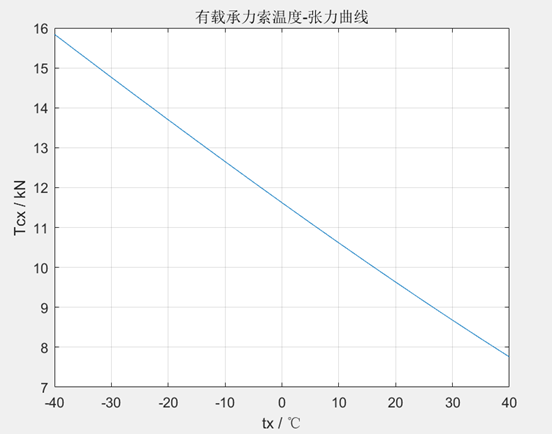
\includegraphics[width=0.7\linewidth]{figures/有载承力索张力-温度曲线}
	\caption{有载承力索张力-温度曲线}
	\label{fig:有载承力索张力-温度曲线}
\end{figure}

\subsection{有载承力索的驰度-温度曲线}
有载承力索的弛度$F_x$与张力$T_{cx}$存在如下关系:
$$
F_x=\frac{W_xl_{i}^{2}}{8Z_x}
$$
上式中,$l_i$表示不同的跨距值,本文中计算跨距分别为35m、40m、45m、50m、55m、60m、65m七种情况下的弛度-温度关系曲线。

分别将上述跨距值代入计算式,利用MATLAB可计算不同跨距下有载承力索的弛度-温度关系,如所示:
\begin{table}[H]
	\centering
	\caption{有载承力索弛度-温度曲线表(跨距为li=35m)}
	\label{tab:有载承力索弛度-温度曲线表(跨距为li=35m)}
	\resizebox{\columnwidth}{!}{%
		\begin{tabular}{|c|c|c|c|c|c|c|c|c|c|}
			\hline
			\textit{tx / ℃} & -40   & -35   & -30   & -25   & -20   & -15   & -10   & -5    & 0     \\ \hline
			\textit{Fx / m} & 0.149 & 0.153 & 0.156 & 0.16  & 0.164 & 0.168 & 0.173 & 0.177 & 0.182 \\ \hline
			\textit{tx / ℃} & 5     & 10    & 15    & 20    & 25    & 30    & 35    & 40    &       \\ \hline
			\textit{Fx / m} & 0.187 & 0.192 & 0.197 & 0.203 & 0.209 & 0.215 & 0.221 & 0.228 &       \\ \hline
		\end{tabular}%
	}
\end{table}
\begin{table}[H]
	\centering
	\caption{有载承力索弛度-温度曲线表(跨距为li=40m)}
	\label{tab:有载承力索弛度-温度曲线表(跨距为li=40m)}
	\resizebox{\columnwidth}{!}{%
		\begin{tabular}{|c|c|c|c|c|c|c|c|c|c|}
			\hline
			\textit{tx / ℃} & -40   & -35   & -30   & -25   & -20   & -15   & -10   & -5    & 0     \\ \hline
			\textit{Fx / m} & 0.195 & 0.199 & 0.204 & 0.209 & 0.214 & 0.22  & 0.225 & 0.231 & 0.238 \\ \hline
			\textit{tx / ℃} & 5     & 10    & 15    & 20    & 25    & 30    & 35    & 40    &       \\ \hline
			\textit{Fx / m} & 0.244 & 0.251 & 0.258 & 0.265 & 0.273 & 0.281 & 0.289 & 0.298 &       \\ \hline
		\end{tabular}%
	}
\end{table}
\begin{table}[H]
	\centering
	\caption{有载承力索弛度-温度曲线表(跨距为li=45m)}
	\label{tab:有载承力索弛度-温度曲线表(跨距为li=45m)}
	\resizebox{\columnwidth}{!}{%
		\begin{tabular}{|c|c|c|c|c|c|c|c|c|c|}
			\hline
			\textit{tx / ℃} & -40   & -35   & -30   & -25   & -20   & -15   & -10   & -5    & 0     \\ \hline
			\textit{Fx / m} & 0.246 & 0.252 & 0.258 & 0.265 & 0.271 & 0.278 & 0.285 & 0.293 & 0.301 \\ \hline
			\textit{tx / ℃} & 5     & 10    & 15    & 20    & 25    & 30    & 35    & 40    &       \\ \hline
			\textit{Fx / m} & 0.309 & 0.317 & 0.326 & 0.336 & 0.345 & 0.355 & 0.366 & 0.377 &       \\ \hline
		\end{tabular}%
	}
\end{table}
\begin{table}[H]
	\centering
	\caption{有载承力索弛度-温度曲线表(跨距为li=50m)}
	\label{tab:有载承力索弛度-温度曲线表(跨距为li=50m)}
	\resizebox{\columnwidth}{!}{%
		\begin{tabular}{|c|c|c|c|c|c|c|c|c|c|}
			\hline
			\textit{tx / ℃} & -40   & -35   & -30   & -25   & -20   & -15   & -10   & -5    & 0     \\ \hline
			\textit{Fx / m} & 0.304 & 0.311 & 0.319 & 0.327 & 0.335 & 0.343 & 0.352 & 0.362 & 0.371 \\ \hline
			\textit{tx / ℃} & 5     & 10    & 15    & 20    & 25    & 30    & 35    & 40    &       \\ \hline
			\textit{Fx / m} & 0.381 & 0.392 & 0.403 & 0.414 & 0.426 & 0.439 & 0.452 & 0.465 &       \\ \hline
		\end{tabular}%
	}
\end{table}
\begin{table}[H]
	\centering
	\caption{有载承力索弛度-温度曲线表(跨距为li=55m)}
	\label{tab:有载承力索弛度-温度曲线表(跨距为li=55m)}
	\resizebox{\columnwidth}{!}{%
		\begin{tabular}{|c|c|c|c|c|c|c|c|c|c|}
			\hline
			\textit{tx / ℃} & -40   & -35   & -30   & -25   & -20   & -15   & -10   & -5    & 0     \\ \hline
			\textit{Fx / m} & 0.368 & 0.377 & 0.386 & 0.395 & 0.405 & 0.416 & 0.426 & 0.438 & 0.449 \\ \hline
			\textit{tx / ℃} & 5     & 10    & 15    & 20    & 25    & 30    & 35    & 40    &       \\ \hline
			\textit{Fx / m} & 0.461 & 0.474 & 0.488 & 0.501 & 0.516 & 0.531 & 0.547 & 0.563 &       \\ \hline
		\end{tabular}%
	}
\end{table}
\begin{table}[H]
	\centering
	\caption{有载承力索弛度-温度曲线表(跨距为li=60m)}
	\label{tab:有载承力索弛度-温度曲线表(跨距为li=60m)}
	\resizebox{\columnwidth}{!}{%
		\begin{tabular}{|c|c|c|c|c|c|c|c|c|c|}
			\hline
			\textit{tx / ℃} & -40   & -35   & -30   & -25   & -20   & -15   & -10   & -5    & 0     \\ \hline
			\textit{Fx / m} & 0.438 & 0.448 & 0.459 & 0.471 & 0.482 & 0.495 & 0.507 & 0.521 & 0.535 \\ \hline
			\textit{tx / ℃} & 5     & 10    & 15    & 20    & 25    & 30    & 35    & 40    &       \\ \hline
			\textit{Fx / m} & 0.549 & 0.564 & 0.58  & 0.597 & 0.614 & 0.632 & 0.651 & 0.67  &       \\ \hline
		\end{tabular}%
	}
\end{table}
\begin{table}[H]
	\centering
	\caption{有载承力索弛度-温度曲线表(跨距为li=65m)}
	\label{tab:有载承力索弛度-温度曲线表(跨距为li=65m)}
	\resizebox{\columnwidth}{!}{%
		\begin{tabular}{|c|c|c|c|c|c|c|c|c|c|}
			\hline
			\textit{tx / ℃} & -40   & -35   & -30   & -25   & -20   & -15   & -10   & -5    & 0     \\ \hline
			\textit{Fx / m} & 0.514 & 0.526 & 0.539 & 0.552 & 0.566 & 0.58  & 0.595 & 0.611 & 0.627 \\ \hline
			\textit{tx / ℃} & 5     & 10    & 15    & 20    & 25    & 30    & 35    & 40    &       \\ \hline
			\textit{Fx / m} & 0.644 & 0.662 & 0.681 & 0.7   & 0.72  & 0.742 & 0.763 & 0.786 &       \\ \hline
		\end{tabular}%
	}
\end{table}
利用MATLAB对有载承力索弛度-温度曲线进行作图,得到如\ref{fig:-有载承力索弛度-温度曲线}所示关系曲线。
% TODO: \usepackage{graphicx} required
\begin{figure}[h]
	\centering
	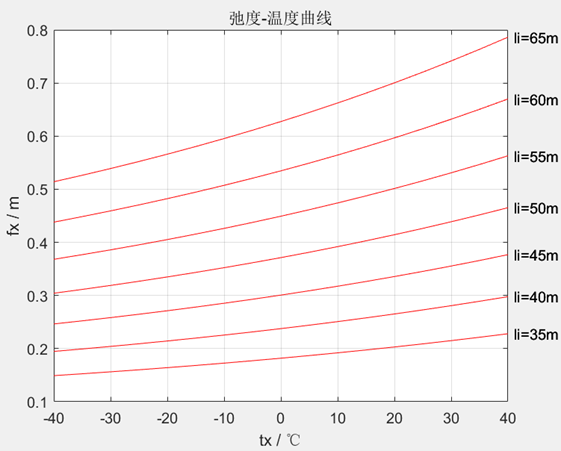
\includegraphics[width=0.7\linewidth]{figures/有载承力索弛度-温度曲线}
	\caption{有载承力索弛度-温度曲线}
	\label{fig:-有载承力索弛度-温度曲线}
\end{figure}

\subsection{接触线的弛度-温度曲线}
接触线的弛度fx与结构系数$\phi$、有载承力索的弛度$F_x$、计算跨距$l_i$存在如下关系:
$$
f_x=\varphi (F_x-F_0)
$$
其中,
\begin{align*}
	F_0&=\frac{q_0l_{i}^{2}}{8T_{c0}}
	\\
	&=\frac{13.91\times 10^{-3}\times l_{i}^{2}}{8\times 11.85}
	\\
	&=1.47\times 10^{-4}l_{i}^{2}
\end{align*}
上式中,计算跨距$l_i$分别取为35m、40m、45m、50m、55m、60m、65m七种情况下的弛度-温度关系曲线。

利用MATLAB对接触线弛度-温度曲线进行作图,得到如\ref{fig:-接触线弛度-温度曲线}所示关系曲线。
% TODO: \usepackage{graphicx} required
\begin{figure}[H]
	\centering
	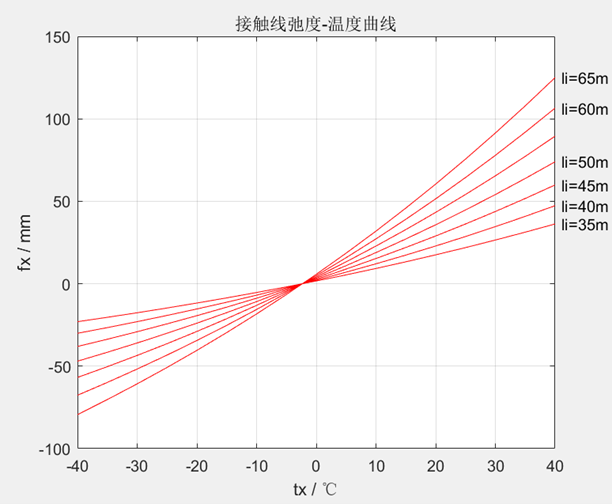
\includegraphics[width=0.7\linewidth]{figures/接触线弛度-温度曲线}
	\caption{接触线弛度-温度曲线}
	\label{fig:-接触线弛度-温度曲线}
\end{figure}

\subsection{接触线的在悬挂点处的高度变化曲线}
接触线在悬挂点处的高度变化$\Delta h_x$与结构系数$\phi$、有载承力索的弛度$F_x$、计算跨距$l_i$存在如下关系:
$$
\varDelta h_x=(1-\varphi )(F_x-F_0)
$$
其中,根据前文可得$F_0=1.47×10^{-4}l^2_i$。
分别取计算跨距li为35m、40m、45m、50m、55m、60m、65m代入计算式,利用MATLAB可计算不同跨距下接触线在悬挂点处变化高度-温度关系,如所示:

% Please add the following required packages to your document preamble:
% \usepackage{graphicx}
\begin{table}[H]
	\centering
	\caption{接触线在悬挂点处变化高度-温度曲线表(跨距为li=35m)}
	\label{tab:my-table}
	\resizebox{\columnwidth}{!}{%
		\begin{tabular}{|c|c|c|c|c|c|c|c|c|c|}
			\hline
			\textit{\textbf{tx / ℃}} & -40   & -35   & -30   & -25   & -20   & -15   & -10   & -5    & 0    \\ \hline
			\textit{fx / mm}         & -7.63 & -6.75 & -5.84 & -4.88 & -3.89 & -2.85 & -1.76 & -0.63 & 0.55 \\ \hline
			\textit{tx / ℃}          & 5     & 10    & 15    & 20    & 25    & 30    & 35    & 40    &      \\ \hline
			\textit{fx / mm}         & 1.78  & 3.07  & 4.41  & 5.81  & 7.27  & 8.79  & 10.37 & 12.02 &      \\ \hline
		\end{tabular}%
	}
\end{table}

% Please add the following required packages to your document preamble:
% \usepackage{graphicx}
\begin{table}[H]
	\centering
	\caption{接触线在悬挂点处变化高度-温度曲线表(跨距为li=40m)}
	\label{tab:my-table}
	\resizebox{\columnwidth}{!}{%
		\begin{tabular}{|c|c|c|c|c|c|c|c|c|c|}
			\hline
			\textit{\textbf{tx / ℃}} & -40  & -35  & -30  & -25  & -20  & -15   & -10   & -5    & 0 \\ \hline
			\textit{fx / mm} & -9.97 & -8.82 & -7.62 & -6.38 & -5.07 & -3.72 & -2.3 & \multicolumn{1}{l|}{-0.82} & 0.72 \\ \hline
			\textit{tx / ℃}          & 5    & 10   & 15   & 20   & 25   & 30    & 35    & 40    &   \\ \hline
			\textit{fx / mm}         & 2.33 & 4.01 & 5.76 & 7.59 & 9.49 & 11.48 & 13.54 & 15.69 &   \\ \hline
		\end{tabular}%
	}
\end{table}

% Please add the following required packages to your document preamble:
% \usepackage{graphicx}
\begin{table}[H]
	\centering
	\caption{接触线在悬挂点处变化高度-温度曲线表(跨距为li=45m)}
	\label{tab:my-table}
	\resizebox{\columnwidth}{!}{%
		\begin{tabular}{|c|c|c|c|c|c|c|c|c|c|}
			\hline
			\textit{\textbf{tx / ℃}} & -40  & -35  & -30  & -25 & -20   & -15   & -10   & -5    & 0 \\ \hline
			\textit{fx / mm} & -12.62 & -11.16 & -9.65 & -8.07 & -6.42 & -4.71 & -2.91 & \multicolumn{1}{l|}{-1.04} & 0.91 \\ \hline
			\textit{tx / ℃}          & 5    & 10   & 15   & 20  & 25    & 30    & 35    & 40    &   \\ \hline
			\textit{fx / mm}         & 2.95 & 5.07 & 7.29 & 9.6 & 12.01 & 14.53 & 17.14 & 19.86 &   \\ \hline
		\end{tabular}%
	}
\end{table}
% Please add the following required packages to your document preamble:
% \usepackage{graphicx}
\begin{table}[H]
	\centering
	\caption{接触线在悬挂点处变化高度-温度曲线表(跨距为li=50m)}
	\label{tab:my-table}
	\resizebox{\columnwidth}{!}{%
		\begin{tabular}{|c|c|c|c|c|c|c|c|c|c|}
			\hline
			\textit{\textbf{tx / ℃}} & -40  & -35  & -30 & -25   & -20   & -15   & -10   & -5    & 0 \\ \hline
			\textit{fx / mm} & -15.58 & -13.78 & -11.91 & -9.96 & -7.93 & -5.81 & -3.6 & \multicolumn{1}{l|}{-1.29} & 1.12 \\ \hline
			\textit{tx / ℃}          & 5    & 10   & 15  & 20    & 25    & 30    & 35    & 40    &   \\ \hline
			\textit{fx / mm}         & 3.64 & 6.26 & 9   & 11.85 & 14.83 & 17.93 & 21.16 & 24.52 &   \\ \hline
		\end{tabular}%
	}
\end{table}
% Please add the following required packages to your document preamble:
% \usepackage{graphicx}
\begin{table}[H]
	\centering
	\caption{接触线在悬挂点处变化高度-温度曲线表(跨距为li=55m)}
	\label{tab:my-table}
	\resizebox{\columnwidth}{!}{%
		\begin{tabular}{|c|c|c|c|c|c|c|c|c|c|}
			\hline
			\textit{\textbf{tx / ℃}} & -40 & -35  & -30   & -25   & -20   & -15  & -10   & -5    & 0 \\ \hline
			\textit{fx / mm} & -18.85 & -16.68 & -14.41 & -12.05 & -9.59 & -7.03 & -4.35 & \multicolumn{1}{l|}{-1.56} & 1.36 \\ \hline
			\textit{tx / ℃}          & 5   & 10   & 15    & 20    & 25    & 30   & 35    & 40    &   \\ \hline
			\textit{fx / mm}         & 4.4 & 7.58 & 10.89 & 14.34 & 17.95 & 21.7 & 25.61 & 29.67 &   \\ \hline
		\end{tabular}%
	}
\end{table}
% Please add the following required packages to your document preamble:
% \usepackage{graphicx}
\begin{table}[H]
	\centering
	\caption{接触线在悬挂点处变化高度-温度曲线表(跨距为li=60m)}
	\label{tab:my-table}
	\resizebox{\columnwidth}{!}{%
		\begin{tabular}{|c|c|c|c|c|c|c|c|c|c|}
			\hline
			\textit{\textbf{tx / ℃}} & -40  & -35  & -30   & -25   & -20   & -15   & -10   & -5    & 0 \\ \hline
			\textit{fx / mm} & -22.43 & -19.85 & -17.15 & -14.35 & -11.42 & -8.36 & -5.18 & \multicolumn{1}{l|}{-1.85} & 1.62 \\ \hline
			\textit{tx / ℃}          & 5    & 10   & 15    & 20    & 25    & 30    & 35    & 40    &   \\ \hline
			\textit{fx / mm}         & 5.24 & 9.02 & 12.96 & 17.07 & 21.36 & 25.82 & 30.47 & 35.31 &   \\ \hline
		\end{tabular}%
	}
\end{table}
% Please add the following required packages to your document preamble:
% \usepackage{graphicx}
\begin{table}[H]
	\centering
	\caption{接触线在悬挂点处变化高度-温度曲线表(跨距为li=65m)}
	\label{tab:my-table}
	\resizebox{\columnwidth}{!}{%
		\begin{tabular}{|c|c|c|c|c|c|c|c|c|c|}
			\hline
			\textit{\textbf{tx / ℃}} & -40  & -35   & -30   & -25   & -20   & -15   & -10   & -5    & 0 \\ \hline
			\textit{fx / mm} & -26.32 & -23.29 & -20.13 & -16.84 & -13.4 & -9.82 & -6.08 & \multicolumn{1}{l|}{-2.17} & 1.9 \\ \hline
			\textit{tx / ℃}          & 5    & 10    & 15    & 20    & 25    & 30    & 35    & 40    &   \\ \hline
			\textit{fx / mm}         & 6.15 & 10.58 & 15.21 & 20.03 & 25.07 & 30.31 & 35.76 & 41.44 &   \\ \hline
		\end{tabular}%
	}
\end{table}
利用MATLAB对接触线在悬挂点处变化高度-温度曲线进行作图,得到如\ref{fig:-接触线在悬挂点处变化高度-温度曲线}所示关系曲线。
% TODO: \usepackage{graphicx} required
\begin{figure}[h]
	\centering
	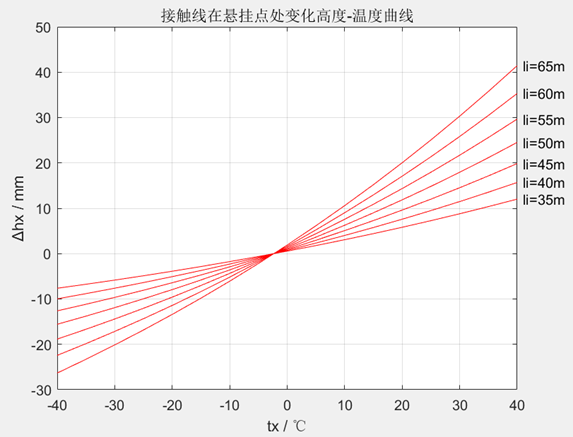
\includegraphics[width=0.7\linewidth]{figures/接触线在悬挂点处变化高度-温度曲线}
	\caption{接触线在悬挂点处变化高度-温度曲线}
	\label{fig:-接触线在悬挂点处变化高度-温度曲线}
\end{figure}

\subsection{无载部分接触线无弛度时承力索张力}
无载部分接触线无弛度时承力索张力$T_{cw0}$与有载部分接触线无弛度时承力索张力$T_{c0}$存在如下关系:
$$
T_{cw0}-\frac{g_{c}^{2}l_{D}^{2}ES}{24T_{cw0}^{2}}=T_{c0}-\frac{q_{0}^{2}l_{D}^{2}ES}{24T_{c0}^{2}}
$$
由前文可得$gc=5.876×10^{-3} kN/m$,计算得到的$T_{c0}=11.85 kN$,利用MATLAB求解得到无载部分接触线无弛度时承力索张力$T_{cw0}=10.73 kN$。
\subsection{无载承力索的张力-温度曲线}
无载承力索张力-温度曲线计算式为:
$$
t_x=[t_0-\frac{g_{c}^{2}l_{D}^{2}}{24\alpha T_{cw0}^{2}}+\frac{T_{cw0}}{\alpha ES}]+\frac{g_{c}^{2}l_{D}^{2}}{24\alpha T_{cwx}^{2}}-\frac{T_{cwx}}{\alpha ES}
$$
上式中$T_{cw0}$为无载承力索在温度$t_0$时的张力,可得$T_{cw0}=10.73kN$;$T_{cwx}$为无载承力索在任意温度时的张力,kN;$g_c$为无载承力索的单位荷载,可得$g_c=5.876×10^{-3} kN/m$;承力索线胀系数为$\alpha=17×10^{-6} m/℃$;悬挂线索弹性模量为$E=105GPa$;悬挂线索横截面积为$S=65.81mm^2$。
利用MATLAB编程求解得到不同温度下无载承力索张力大小,如\ref{tab:无载承力索张力-温度曲线表}所示:
% Please add the following required packages to your document preamble:
% \usepackage{graphicx}
\begin{table}[h]
	\centering
	\caption{无载承力索张力-温度曲线表}
	\label{tab:无载承力索张力-温度曲线表}
	\resizebox{\columnwidth}{!}{%
		\begin{tabular}{|c|c|c|c|c|c|c|c|c|c|}
			\hline
			\textit{tx / ℃}   & -40   & -30   & -20   & -10   & 0    & 10   & 20   & 30   & 40   \\ \hline
			\textit{Tcx / kN} & 14.12 & 12.98 & 11.88 & 10.73 & 9.63 & 8.56 & 7.53 & 6.55 & 5.66 \\ \hline
		\end{tabular}%
	}
\end{table}
利用MATLAB对有载承力索张力-温度曲线进行作图,得到如\ref{fig:-无载承力索张力-温度曲线}所示关系曲线。
% TODO: \usepackage{graphicx} required
\begin{figure}[H]
	\centering
	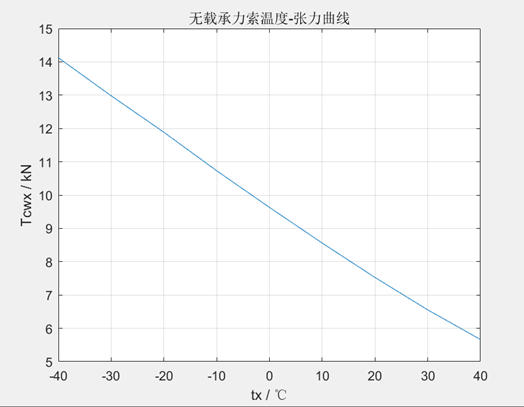
\includegraphics[width=0.7\linewidth]{figures/无载承力索张力-温度曲线}
	\caption{无载承力索张力-温度曲线}
	\label{fig:-无载承力索张力-温度曲线}
\end{figure}

\subsection{无载承力索的弛度-温度曲线}
无载承力索的弛度$F_{wx}$与张力$T_{cwx}$存在如下关系:
$$
F_{wx}=\frac{g_cl_{i}^{2}}{8T_{cwx}}
$$
上式中,计算跨距$l_i$分别取为35m、40m、45m、50m、55m、60m、65m七种情况下的弛度-温度关系曲线。

分别将上述跨距值代入计算式,利用MATLAB可计算不同跨距下无载承力索的弛度-温度关系,如表2-9所示:





利用MATLAB对无载承力索弛度-温度曲线进行作图,得到\ref{fig:-无载承力索弛度-温度曲线}所示关系曲线。

% TODO: \usepackage{graphicx} required
\begin{figure}[h]
	\centering
	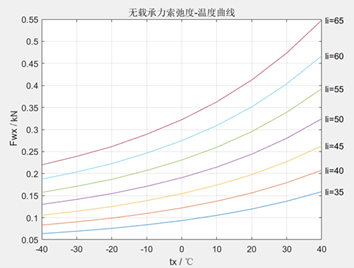
\includegraphics[width=0.7\linewidth]{figures/无载承力索弛度-温度曲线}
	\caption{无载承力索弛度-温度曲线}
	\label{fig:-无载承力索弛度-温度曲线}
\end{figure}

\section{半补偿链形悬挂锚段长度及张力增量曲线确定}
\subsection{计算条件}
工程设计中规定在计算极限温度下,中心锚结处补偿器张力差值$\Delta T\leqslant \pm 15\%T_j$。其中,$T_j$代表接触线在补偿器处的张力。

对于JT-95型承力索,其线胀系数为$\alpha_c=17×10^{-6} m/℃$,弹性模量为$Ec=105GPa$;悬挂线索横截面积为$Sc=65.81mm^2$;而对于站线接触线,其选用CT-110型线索,该线索线胀系数为$\alpha_j=17×10^{-6}m/℃$,弹性模量为$Ej=120GPa$;悬挂线索横截面积为$Sc=86mm^2$。

吊弦及定位器处于正常位置时的温度为:
\begin{align*}
	t_d&=\frac{t_{\max}+t_{\min}}{2}
	\\
	&=\frac{40-40}{2}
	\\
	&=0^{\circ}C
\end{align*}
根据上式可知温差为$|\Delta t_1|=|\Delta t_2|=40^{\circ}C$;由原始资料可知,结构高度取为$h=1.6m$。

接触线无弛度时承力索弛度为:
\begin{align*}
	F_0&=\frac{q_0l_{D}^{2}}{8T_{c0}}
	\\
	&=\frac{13.91\times 10^{-3}\times 60^2}{8\times 11.85}
	\\
	&=0.528m
\end{align*}
吊弦平均长度为:
\begin{align*}
	C&=h-\frac{2}{3}F_0
	\\
	&=1.6-\frac{2}{3}\times 0.528
	\\
	&=1.248m
\end{align*}

\subsection{吊弦造成的张力增量}
吊弦在直线区段造成的张力增量计算式如下:
$$
\varDelta T_{jd}=\frac{L(L+l)g_j(\alpha _j\varDelta t-\varepsilon )}{2C}
$$
上式中,$\Delta T_{jd}$为只考虑温度变化时,吊弦所引起的张力增量,kN;L为由中心锚结至补偿器间的距离,取为半锚段长度,m;C为吊弦平均长度,m;l为锚段长度,直线区段取为65m;$\Delta t$为最低温度与吊弦及定位器处于正常位置时温度的差值的绝对值,$\Delta t=40℃$;$\epsilon$是一个非常小的数,一般不用考虑,下文计算中均将其作为零值处理。

计算得到半锚段长度不同时吊弦造成的张力增量的大小,其计算结果如\ref{tab:直线区段(l=65m)吊弦造成的张力增量ΔTjd与L的关系数据表(-40℃)}所示。
% Please add the following required packages to your document preamble:
% \usepackage{graphicx}
\begin{table}[H]
	\centering
	\caption{直线区段(l=65m)吊弦造成的张力增量ΔTjd与L的关系数据表(-40℃)
	}
	\label{tab:直线区段(l=65m)吊弦造成的张力增量ΔTjd与L的关系数据表(-40℃)}
	\resizebox{\columnwidth}{!}{%
		\begin{tabular}{|l|c|c|c|c|c|c|c|c|c|}
			\hline
			\multicolumn{1}{|c|}{\textit{L / m}} & 200   & 300   & 400   & 500  & 600   & 700   & 800  & 900   & 40   \\ \hline
			\textit{ΔTjd / kN}                   & 0.109 & 0.225 & 0.382 & 0.58 & 0.819 & 1.099 & 1.42 & 1.783 & 5.66 \\ \hline
		\end{tabular}%
	}
\end{table}

\subsection{定位器造成的张力增量}
定位器在曲线区段造成的张力增量计算式如下:
$$
\Delta T_{j_{iv}}=\frac{L(L-l)\alpha _j\Delta t}{2Rd+0.5L(L-l)\alpha _j\Delta t}(T_{jmax}+\frac{2}{3}\Delta T_{ja})
$$
上式中,$\Delta T_{jw}$为只考虑温度变化时,定位器所引起的张力增量,kN;R为曲线区段的曲率半径,m;d为定位器长度,取为1.2m;$\Delta T_{jd}$大小见前文;其它各参数物理意义与前文中吊弦造成的张力增量计算式中的含义相同。

计算得到不同曲率半径下半锚段长度及曲率半径与吊弦造成的张力增量之间的关系,如\ref{tab:定位器引起的张力增量ΔTjw与L、R的关系数据表(-40℃)}所示。
\begin{table}[h]
	\centering
	\caption{定位器引起的张力增量ΔTjw与L、R的关系数据表(-40℃)}
	\label{tab:定位器引起的张力增量ΔTjw与L、R的关系数据表(-40℃)}
	\resizebox{\columnwidth}{!}{%
		\begin{tabular}{|c|c|c|c|c|c|c|}
			\hline
			\textit{ΔTjw / kN} & \multicolumn{1}{c|}{\textit{R=300m}} & \multicolumn{1}{c|}{\textit{R=400m}} & \multicolumn{1}{c|}{\textit{R=500m}} & \multicolumn{1}{c|}{\textit{R=600m}} & \multicolumn{1}{c|}{\textit{R=2000m}} & \multicolumn{1}{c|}{\textit{R=3000m}} \\ \hline
			\textit{L=200m} & 0.2536 & 0.1908 & 0.1529 & 0.1276 & 0.0385 & 0.0257 \\ \hline
			\textit{L=300m} & 0.654 & 0.4945 & 0.3975 & 0.3324 & 0.1009 & 0.0674 \\ \hline
			\textit{L=400m} & 1.2205 & 0.9292 & 0.7502 & 0.629 & 0.1928 & 0.129 \\ \hline
			\textit{L=500m} & 1.9348 & 1.4857 & 1.2058 & 1.0147 & 0.3152 & 0.2112 \\ \hline
			\textit{L=600m} & 2.7763 & 2.1531 & 1.7584 & 1.486 & 0.4689 & 0.3149 \\ \hline
			\textit{L=700m} & 3.724 & 2.9196 & 2.401 & 2.0389 & 0.6552 & 0.4413 \\ \hline
			\textit{L=800m} & 4.758 & 3.7735 & 3.1266 & 2.669 & 0.8754 & 0.5915 \\ \hline
			\textit{L=900m} & 5.861 & 4.7038 & 3.9282 & 3.3721 & 1.1309 & 0.7669 \\ \hline
		\end{tabular}%
	}
\end{table}

\subsection{直线区段张力差计算}
直线区段的张力差取决于吊弦造成的张力增量及温度等因素引起的弹性伸长量,其计算式如下:
$$
\varDelta T_{jdE}=\frac{L(L+l)g_j\alpha _j\varDelta t}{2C+\frac{2}{3}\frac{L(L+l)}{E_jS_j}g_j}
$$
计算得到半锚段长度不同时直线区段张力差的大小,其结果如\ref{tab:直线区段(l=65m)吊弦造成的张力增量ΔTjd与L的关系数据表(-40℃)}所示。
% Please add the following required packages to your document preamble:
% \usepackage{graphicx}
\begin{table}[h]
	\centering
	\caption{直线区段(l=65m)张力差ΔTjdE与L的关系数据表(-40℃)
	}
	\label{tab:直线区段(l=65m)张力差ΔTjdE与L的关系数据表(-40℃)}
	\resizebox{\columnwidth}{!}{%
		\begin{tabular}{|c|c|c|c|c|c|c|c|c|}
			\hline
			\textit{L / m} & 200    & 300    & 400    & 500    & 600    & 700    & 800    & 900    \\ \hline
			ΔTjdE / kN     & 0.1077 & 0.2201 & 0.3684 & 0.5496 & 0.7598 & 0.9952 & 1.2515 & 1.5245 \\ \hline
		\end{tabular}%
	}
\end{table}


